\documentclass[12pt]{article}
\usepackage[a4paper, total={6in, 9in}]{geometry}
\usepackage{graphicx}
\graphicspath{ {./images/output/} }
\usepackage{caption}
\usepackage[english]{babel}
\usepackage{titling}
\usepackage{float}
% \usepackage{amsmath}
% \usepackage{minted}
% \usepackage{multicol}
% \usepackage{array}
% \usepackage{setspace}
% \usepackage{placeins}

% \usepackage{lipsum}

\title{Different types of commands in AutoCAD Electrical}
\author{}
\date{}

\pagenumbering{gobble}
\begin{document}
\vspace*{\fill}
\begin{center}

    \emph{Heaven's Light is Our Guide} \\
    \textbf{Rajshahi University of Engineering and Technology} \\

    \begin{figure}[H]
        \centering
        
\includegraphics[scale=.34]{images/RUET_logo.png}
        \label{fig:ruet_logo}
    \end{figure}
    \vspace{5mm}

    \textbf{Course Code}\\
    ECE 3206\\
    \vspace{3mm}
    \textbf{Course Title}\\
    Industrial Electronics Sessional

    \vspace{5mm}
    \textbf{Experiment Date:} {November 24, 2024},\\
    \textbf{Submission Date:} {December 9, 2024}\\

    \vspace{5mm}
    \textbf{Lab Report 1: \\
        Basics of Oscilloscope and Signal Generator}

    \vspace{15mm}

    \begin{tabular}{c|c}
        \textbf{Submitted to} & \textbf{Submitted by} \\
        Md. Faysal Ahamed     & Md. Tajim An Noor     \\
        Lecturer              & Roll: 2010025         \\
        Dept of ECE, Ruet     &                       \\
    \end{tabular}

\end{center}
\vspace*{\fill}


\pagebreak

\tableofcontents

\pagebreak
\pagenumbering{arabic}
\maketitle

\section*{Theory}
\addcontentsline{toc}{section}{Theory}
AutoCAD Electrical has a number of commands that are used to create and modify electrical drawings. These commands help in creating accurate and efficient electrical designs. Understanding and mastering these commands can significantly improve productivity and ensure the quality of the electrical drawings. Additionally, AutoCAD Electrical provides tools for automating repetitive tasks, which can save time and reduce errors. The software also supports collaboration among team members by allowing multiple users to work on the same project simultaneously.

Furthermore, AutoCAD Electrical supports the creation of intelligent electrical symbols and components, which can be reused across different projects. This helps in maintaining consistency and standardization in electrical designs. The software also includes a comprehensive library of electrical symbols and components, which can be easily accessed and inserted into the drawings. Overall, AutoCAD Electrical is a powerful tool for electrical design and drafting, offering a wide range of features and commands to streamline the design process and enhance productivity.

\section*{Different types of commands in AutoCAD Electrical}
\addcontentsline{toc}{section}{Different types of commands in AutoCAD Electrical}
Some of the key commands in AutoCAD Electrical include basic drawing tools, editing tools, layer management, symbol insertion, wire numbering, and schematic creation. These commands are essential for efficient and accurate electrical design. Here are some of the most commonly used commands in AutoCAD Electrical:

\subsection*{1. Line command (L)}
\addcontentsline{toc}{subsection}{Line command (L)}
\begin{description}
    \item [\textbf{Description}] The Line command is used to draw straight lines in the drawing. It is one of the most basic commands in AutoCAD Electrical and is commonly used to create the outlines of electrical components and symbols.
    \item [\textbf{Usage \& Example}] To draw a horizontal line with a length of 10 units, type "L" in the command line and press Enter. Then, specify the start point by clicking on the screen. Next, enter the length of the line as "10" and press Enter. Finally, click on the screen to specify the end point of the line.
          \begin{figure}[H]
              \centering
              % 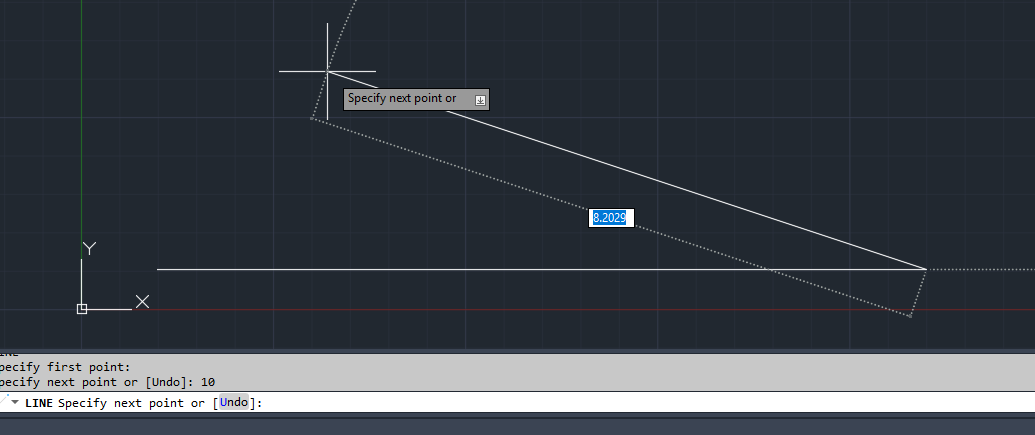
\includegraphics[width=0.5\textwidth]{line_command.png}
              \caption{Line command in AutoCAD Electrical}
          \end{figure}
    \item [\textbf{Significance}] The Line command is essential for creating the basic geometry of electrical drawings. It is used to draw wires, cables, and other linear elements in the drawing. By using the Line command, users can accurately define the layout and dimensions of electrical components and symbols.
\end{description}

\subsection*{2. Polyline command (PL)}
\addcontentsline{toc}{subsection}{Polyline command (PL)}
\begin{description}
    \item [\textbf{Description}] The Polyline command is used to draw a series of connected line segments and arcs in a single object. It is useful for creating complex shapes and paths in the drawing.
    \item [\textbf{Usage \& Example}] To draw a polyline with three segments, type "PL" in the command line and press Enter. Specify the start point by clicking on the screen, then click to specify the next two points. Press Enter to complete the polyline.
          \begin{figure}[H]
              \centering
              % 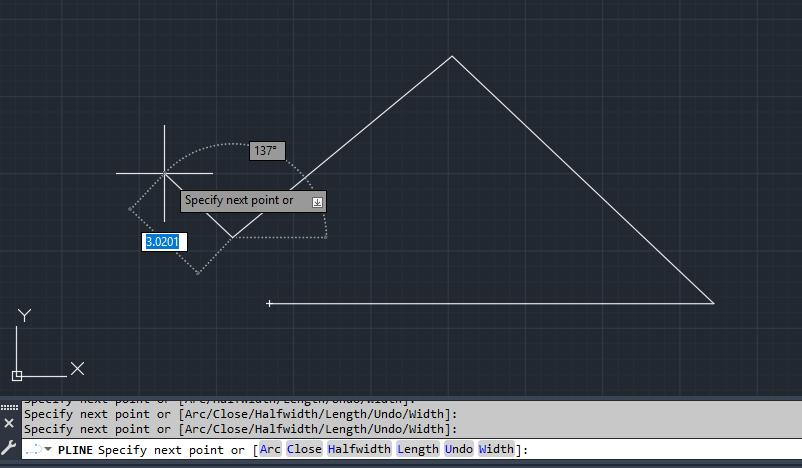
\includegraphics[width=0.5\textwidth]{polyline_command.png}
              \caption{Polyline command in AutoCAD Electrical}
          \end{figure}
    \item [\textbf{Significance}] The Polyline command is essential for creating complex shapes and paths in electrical drawings. It allows users to draw continuous lines with multiple segments, which can be edited as a single object.
\end{description}

\subsection*{3. Circle command (C)}
\addcontentsline{toc}{subsection}{Circle command (C)}
\begin{description}
    \item [\textbf{Description}] The Circle command is used to draw circles in the drawing. It is commonly used to represent round electrical components and symbols.
    \item [\textbf{Usage \& Example}] To draw a circle with a radius of 5 units, type "C" in the command line and press Enter. Specify the center point by clicking on the screen, then enter the radius as "5" and press Enter.
          \begin{figure}[H]
              \centering
              % 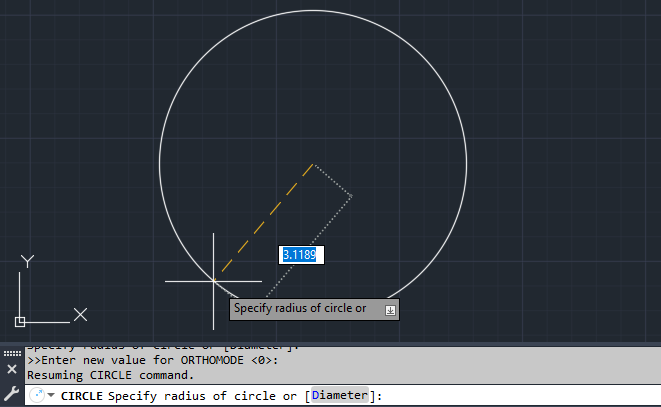
\includegraphics[width=0.5\textwidth]{circle_command.png}
              \caption{Circle command in AutoCAD Electrical}
          \end{figure}
    \item [\textbf{Significance}] The Circle command is essential for creating round shapes and symbols in electrical drawings. It allows users to accurately define the size and position of circular components.
\end{description}

\subsection*{4. Arc command (A)}
\addcontentsline{toc}{subsection}{Arc command (A)}
\begin{description}
    \item [\textbf{Description}] The Arc command is used to draw arcs in the drawing. It is useful for creating curved lines and shapes in electrical drawings.
    \item [\textbf{Usage \& Example}] To draw an arc with a specified start, center, and end point, type "A" in the command line and press Enter. Specify the start point by clicking on the screen, then specify the center point and end point.
          \begin{figure}[H]
              \centering
              % 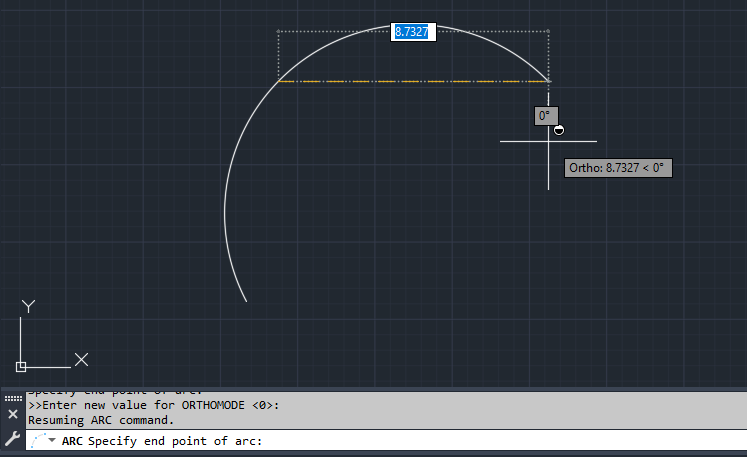
\includegraphics[width=0.5\textwidth]{arc_command.png}
              \caption{Arc command in AutoCAD Electrical}
          \end{figure}
    \item [\textbf{Significance}] The Arc command is essential for creating curved lines and shapes in electrical drawings. It allows users to accurately define the curvature and dimensions of arcs.
\end{description}

\subsection*{5. Move command (M)}
\addcontentsline{toc}{subsection}{Move command (M)}
\begin{description}
    \item [\textbf{Description}] The Move command is used to move objects from one location to another in the drawing. It is useful for repositioning electrical components and symbols.
    \item [\textbf{Usage \& Example}]To move an object from one location to another, type "M" in the command line and press Enter. Select the object to move, specify the base point by clicking on the screen, then specify the destination point.
          \begin{figure}[H]
              \centering
              % 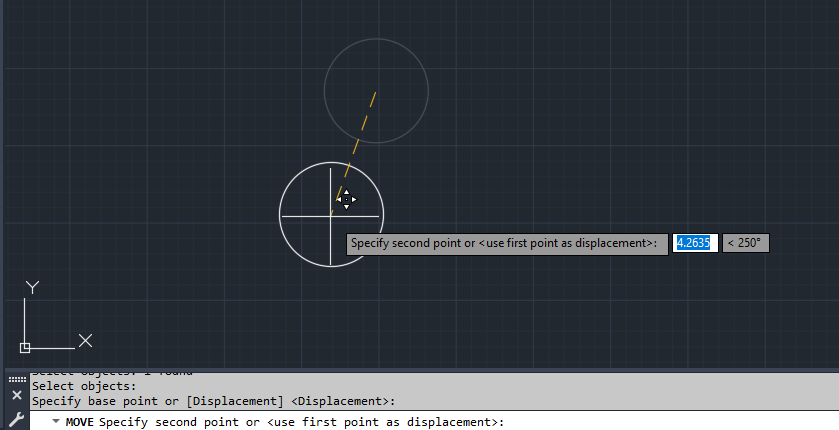
\includegraphics[width=0.5\textwidth]{move_command.png}
              \caption{Move command in AutoCAD Electrical}
          \end{figure}
    \item [\textbf{Significance}] The Move command is essential for repositioning objects in electrical drawings. It allows users to accurately move components and symbols to the desired location.
\end{description}

\subsection*{6. Copy command (CO)}
\addcontentsline{toc}{subsection}{Copy command (CO)}
\begin{description}
    \item [\textbf{Description}] The Copy command is used to create copies of objects in the drawing. It is useful for duplicating electrical components and symbols.
    \item [\textbf{Usage \& Example}] To create a copy of an object, type "CO" in the command line and press Enter. Select the object to copy, specify the base point by clicking on the screen, then specify the destination point.
          \begin{figure}[H]
              \centering
              % 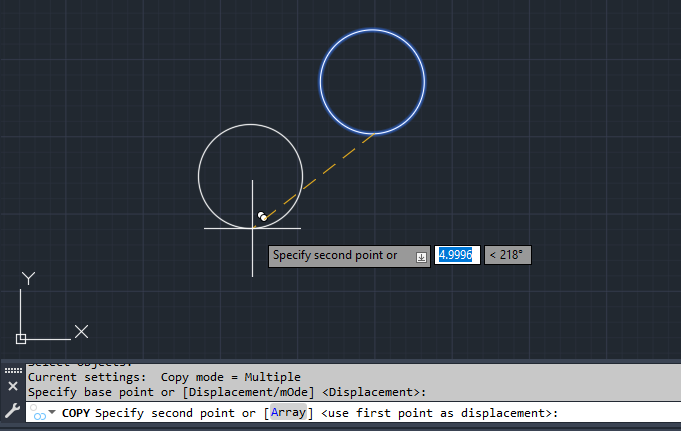
\includegraphics[width=0.5\textwidth]{copy_command.png}
              \caption{Copy command in AutoCAD Electrical}
          \end{figure}
    \item [\textbf{Significance}] The Copy command is essential for duplicating objects in electrical drawings. It allows users to create multiple instances of components and symbols quickly and accurately.
\end{description}

\subsection*{7. Rotate command (RO)}
\addcontentsline{toc}{subsection}{Rotate command (RO)}
\begin{description}
    \item [\textbf{Description}] The Rotate command is used to rotate objects around a specified base point in the drawing. It is useful for changing the orientation of electrical components and symbols.
    \item [\textbf{Usage \& Example}]To rotate an object by 45 degrees, type "RO" in the command line and press Enter. Select the object to rotate, specify the base point by clicking on the screen, then enter the rotation angle as "45" and press Enter.
          \begin{figure}[H]
              \centering
              % 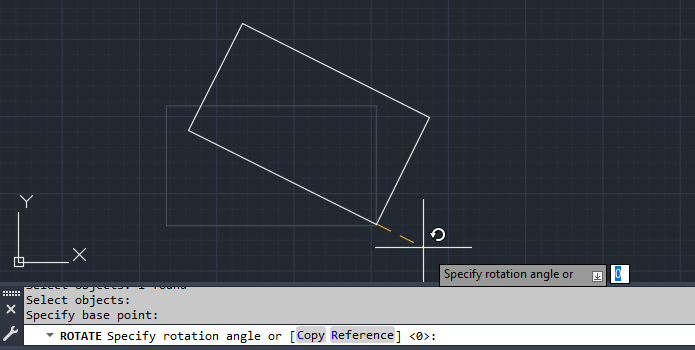
\includegraphics[width=0.5\textwidth]{rotate_command.png}
              \caption{Rotate command in AutoCAD Electrical}
          \end{figure}
    \item [\textbf{Significance}] The Rotate command is essential for changing the orientation of objects in electrical drawings. It allows users to accurately rotate components and symbols to the desired angle.
\end{description}

\subsection*{8. Mirror command (MI)}
\addcontentsline{toc}{subsection}{Mirror command (MI)}
\begin{description}
    \item [\textbf{Description}] The Mirror command is used to create a mirrored copy of objects across a specified axis in the drawing. It is useful for creating symmetrical designs and duplicating components.
    \item [\textbf{Usage \& Example}]To create a mirrored copy of an object, type "MI" in the command line and press Enter. Select the object to mirror, specify the first and second points of the mirror line by clicking on the screen.
          \begin{figure}[H]
              \centering
              % 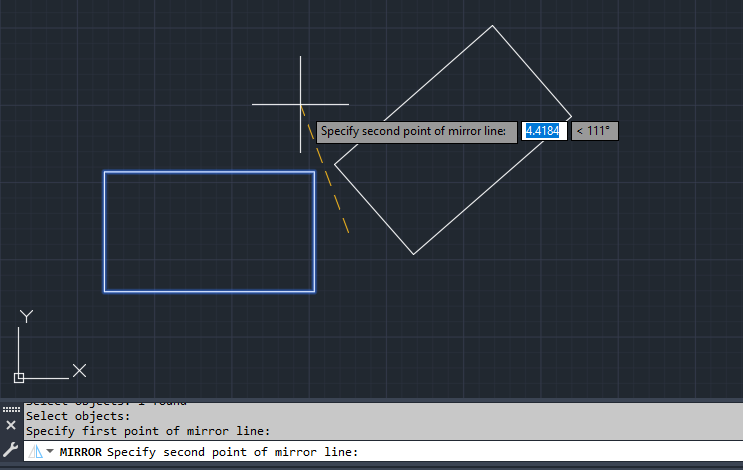
\includegraphics[width=0.5\textwidth]{mirror_command.png}
              \caption{Mirror command in AutoCAD Electrical}
          \end{figure}
    \item [\textbf{Significance}] The Mirror command is essential for creating symmetrical designs and duplicating objects in electrical drawings. It allows users to quickly create mirrored copies of components and symbols.
\end{description}

\subsection*{9. Extend command (EX)}
\addcontentsline{toc}{subsection}{Extend command (EX)}
\begin{description}
    \item [\textbf{Description}] The Extend command is used to extend objects to meet the edges of other objects in the drawing. It is useful for connecting lines and shapes in electrical drawings.
    \item [\textbf{Usage \& Example}] To extend a line to meet another line, type "EX" in the command line and press Enter. Select the boundary edge by clicking on the screen, then select the line to extend.
          \begin{figure}[H]
              \centering
              % 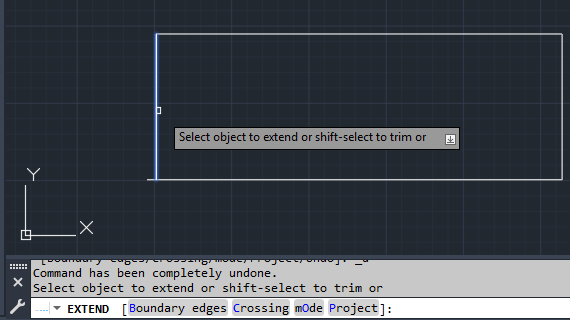
\includegraphics[width=0.5\textwidth]{extend_command.png}
              \caption{Extend command in AutoCAD Electrical}
          \end{figure}
    \item [\textbf{Significance}] The Extend command is essential for connecting lines and shapes in electrical drawings. It allows users to accurately extend objects to meet the desired edges.
\end{description}

\subsection*{10. Trim command (TR)}
\addcontentsline{toc}{subsection}{Trim command (TR)}
\begin{description}
    \item [\textbf{Description}] The Trim command is used to trim objects to meet the edges of other objects in the drawing. It is useful for removing unwanted parts of lines and shapes in electrical drawings.
    \item [\textbf{Usage \& Example}] To trim a line to meet another line, type "TR" in the command line and press Enter. Select the boundary edge by clicking on the screen, then select the line to trim.
          \begin{figure}[H]
              \centering
              % 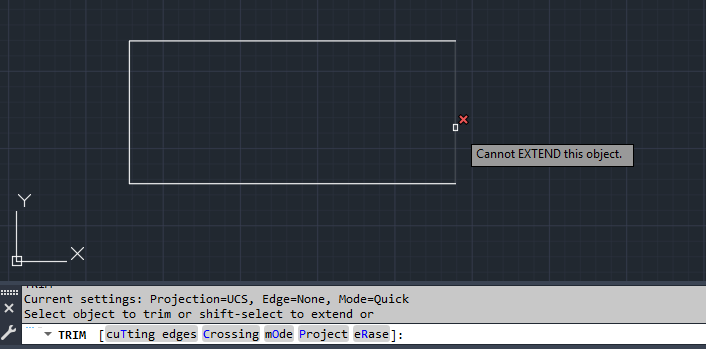
\includegraphics[width=0.5\textwidth]{trim_command.png}
              \caption{Trim command in AutoCAD Electrical}
          \end{figure}
    \item [\textbf{Significance}] The Trim command is essential for removing unwanted parts of lines and shapes in electrical drawings. It allows users to accurately trim objects to meet the desired edges.
\end{description}

\subsection*{11. Erase command (E)}
\addcontentsline{toc}{subsection}{Erase command (E)}
\begin{description}
    \item [\textbf{Description}] The Erase command is used to delete objects from the drawing. It is useful for removing unwanted components and symbols from electrical drawings.
    \item [\textbf{Usage \& Example}]To erase an object, type "E" in the command line and press Enter. Select the object to erase by clicking on the screen, then press Enter to confirm the deletion.
          \begin{figure}[H]
              \centering
              % 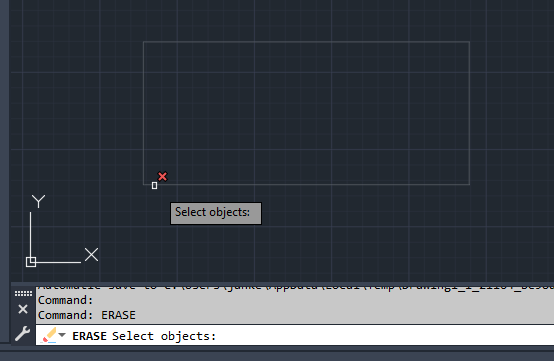
\includegraphics[width=0.5\textwidth]{erase_command.png}
              \caption{Erase command in AutoCAD Electrical}
          \end{figure}
    \item [\textbf{Significance}] The Erase command is essential for removing unwanted objects from electrical drawings. It allows users to clean up the drawing by deleting unnecessary components and symbols.
\end{description}

\subsection*{12. Zoom command (Z)}
\addcontentsline{toc}{subsection}{Zoom command (Z)}
\begin{description}
    \item [\textbf{Description}] The Zoom command is used to change the magnification of the drawing view. It is useful for focusing on specific areas of the drawing.
    \item [\textbf{Usage \& Example}]To zoom into a specific area, type "Z" in the command line and press Enter. Then, type "W" for Window and specify the corners of the zoom window by clicking on the screen.
          \begin{figure}[H]
              \centering
              % 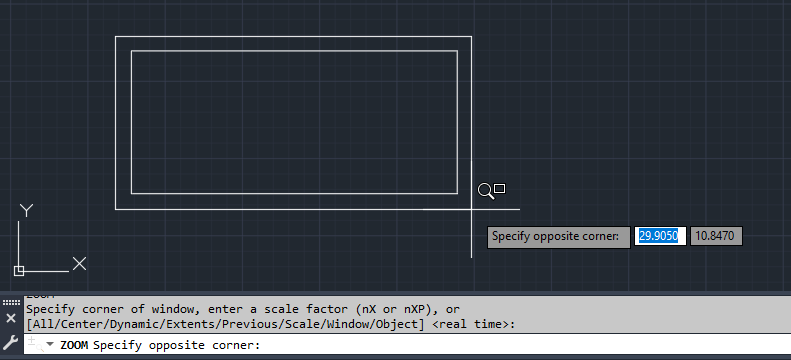
\includegraphics[width=0.5\textwidth]{zoom_command.png}
              \caption{Zoom command in AutoCAD Electrical}
          \end{figure}
    \item [\textbf{Significance}] The Zoom command is essential for navigating and viewing different parts of the drawing. It allows users to focus on details and work more efficiently.
\end{description}

\subsection*{13. Layer command (LA)}
\addcontentsline{toc}{subsection}{Layer command (LA)}
\begin{description}
    \item [\textbf{Description}] The Layer command is used to manage layers in the drawing. It is useful for organizing and controlling the visibility of different elements.
    \item [\textbf{Usage \& Example}] To create a new layer, type "LA" in the command line and press Enter. In the Layer Properties Manager, click on the "New Layer" button and enter the layer name.
          \begin{figure}[H]
              \centering
              % 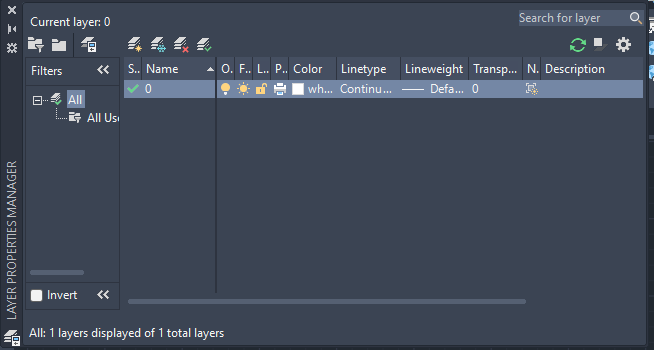
\includegraphics[width=0.5\textwidth]{layer_command.png}
              \caption{Layer command in AutoCAD Electrical}
          \end{figure}
    \item [\textbf{Significance}] The Layer command is essential for organizing the drawing into different categories. It allows users to control the visibility, color, and properties of different elements.
\end{description}

\subsection*{14. Symbol Insert command (X)}
\addcontentsline{toc}{subsection}{Symbol Insert command (X)}
\begin{description}
    \item [\textbf{Description}] The Symbol Insert command is used to insert predefined electrical symbols into the drawing. It is useful for quickly adding standard components.
    \item [\textbf{Usage \& Example}] To insert a resistor symbol, type "X" in the command line and press Enter. Select the resistor symbol from the library and click on the screen to specify the insertion point.
          \begin{figure}[H]
              \centering
              % 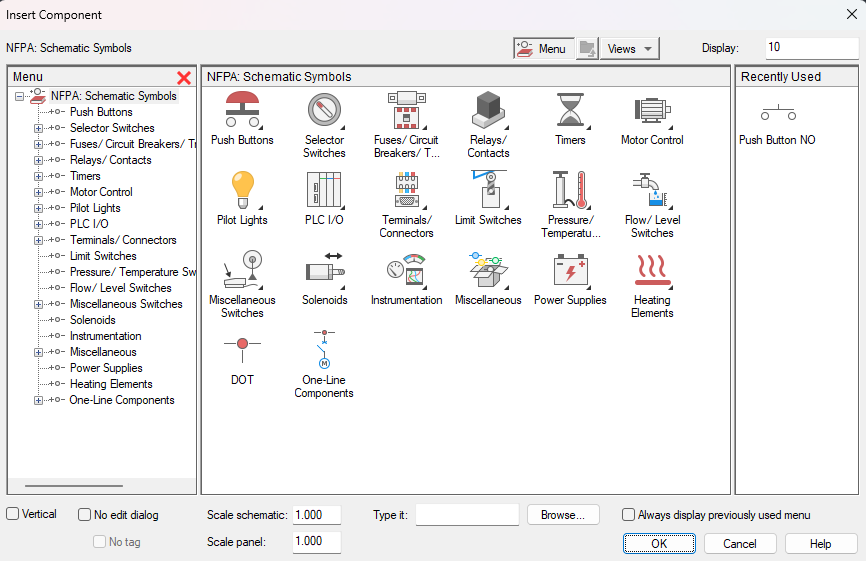
\includegraphics[width=0.5\textwidth]{symbol_insert_command.png}
              \caption{Symbol Insert command in AutoCAD Electrical}
          \end{figure}
    \item [\textbf{Significance}] The Symbol Insert command is essential for adding standard electrical components to the drawing. It ensures consistency and accuracy in the design.
\end{description}

\subsection*{15. Wire Number command (W)}
\addcontentsline{toc}{subsection}{Wire Number command (W)}
\begin{description}
    \item [\textbf{Description}] The Wire Number command is used to assign wire numbers to electrical wires in the drawing. It is useful for identifying and labeling wires.
    \item [\textbf{Usage \& Example}]To assign a wire number to a wire, type "W" in the command line and press Enter. Select the wire by clicking on the screen and enter the wire number.
          \begin{figure}[H]
              \centering
              % 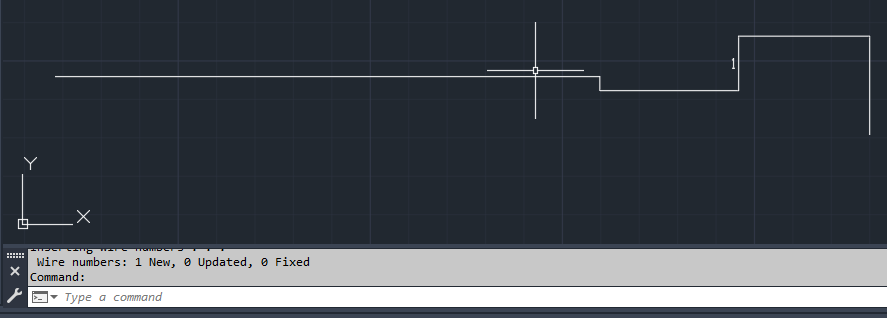
\includegraphics[width=0.5\textwidth]{wire_number_command.png}
              \caption{Wire Number command in AutoCAD Electrical}
          \end{figure}
    \item [\textbf{Significance}] The Wire Number command is essential for labeling and identifying wires in the drawing. It helps in maintaining clarity and organization in the design.
\end{description}

\subsection*{16. Insert Terminal Strip command (ITS)}
\addcontentsline{toc}{subsection}{Insert Terminal Strip command (ITS)}
\begin{description}
    \item [\textbf{Description}] The Insert Terminal Strip command is used to insert terminal strips into the drawing. It is useful for adding terminal connections.
    \item [\textbf{Usage \& Example}] To insert a terminal strip, type "ITS" in the command line and press Enter. Select the terminal strip from the library and click on the screen to specify the insertion point.
          \begin{figure}[H]
              \centering
              % \includegraphics[width=0.5\textwidth]{insert_terminal_strip_command.png}
              \caption{Insert Terminal Strip command in AutoCAD Electrical}
          \end{figure}
    \item [\textbf{Significance}] The Insert Terminal Strip command is essential for adding terminal connections to the drawing. It ensures accurate and organized terminal placements.
\end{description}

\subsection*{17. Create Schematic command (S)}
\addcontentsline{toc}{subsection}{Create Schematic command (S)}
\begin{description}
    \item [\textbf{Description}] The Create Schematic command is used to create electrical schematics in the drawing. It is useful for designing electrical circuits.
    \item [\textbf{Usage \& Example}]To create a simple schematic, type "S" in the command line and press Enter. Use the tools to draw the circuit components and connections.
          \begin{figure}[H]
              \centering
              % 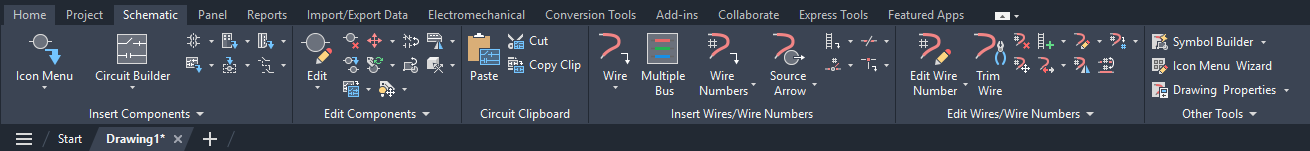
\includegraphics[width=0.5\textwidth]{create_schematic_command.png}
              \caption{Create Schematic command in AutoCAD Electrical}
          \end{figure}
    \item [\textbf{Significance}] The Create Schematic command is essential for designing electrical circuits. It allows users to create detailed and accurate schematics.
\end{description}

\subsection*{18. Cross-reference command (XREF)}
\addcontentsline{toc}{subsection}{Cross-reference command (XREF)}
\begin{description}
    \item [\textbf{Description}] The Cross-reference command is used to create cross-references between different parts of the drawing. It is useful for linking related components.
    \item [\textbf{Usage \& Example}] To create a cross-reference, type "XREF" in the command line and press Enter. Select the objects by clicking on the screen and enter the reference details.
          \begin{figure}[H]
              \centering
              % 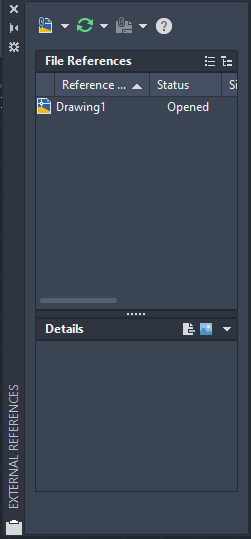
\includegraphics[width=0.5\textwidth]{cross_reference_command.png}
              \caption{Cross-reference command in AutoCAD Electrical}
          \end{figure}
    \item [\textbf{Significance}] The Cross-reference command is essential for linking related components in the drawing. It helps in maintaining clarity and organization.
\end{description}

\subsection*{19. AutoNumber command (AN)}
\addcontentsline{toc}{subsection}{AutoNumber command (AN)}
\begin{description}
    \item [\textbf{Description}] The AutoNumber command is used to automatically assign numbers to components in the drawing. It is useful for numbering and labeling components.
    \item [\textbf{Usage \& Example}] To automatically number components, type "AN" in the command line and press Enter. Select the components by clicking on the screen and specify the numbering options.
          \begin{figure}[H]
              \centering
              % \includegraphics[width=0.5\textwidth]{autonumber_command.png}
              \caption{AutoNumber command in AutoCAD Electrical}
          \end{figure}
    \item [\textbf{Significance}] The AutoNumber command is essential for numbering and labeling components in the drawing. It ensures consistency and accuracy in the design.
\end{description}

\subsection*{20. PLC (Programmable Logic Controller) Wiring command}
\addcontentsline{toc}{subsection}{PLC (Programmable Logic Controller) Wiring command}
\begin{description}
    \item [\textbf{Description}] The PLC Wiring command is used to create wiring diagrams for programmable logic controllers. It is useful for designing PLC circuits.
    \item [\textbf{Usage \& Example}] To create a PLC wiring diagram, type "PLC" in the command line and press Enter. Use the tools to draw the PLC components and connections.
          \begin{figure}[H]
              \centering
              % \includegraphics[width=0.5\textwidth]{plc_wiring_command.png}
              \caption{PLC Wiring command in AutoCAD Electrical}
          \end{figure}
    \item [\textbf{Significance}] The PLC Wiring command is essential for designing PLC circuits. It allows users to create detailed and accurate wiring diagrams.
\end{description}

\subsection*{21. Component Tagging command (CT)}
\addcontentsline{toc}{subsection}{Component Tagging command (CT)}
\begin{description}
    \item [\textbf{Description}] The Component Tagging command is used to assign tags to electrical components in the drawing. It is useful for identifying and labeling components.
    \item [\textbf{Usage \& Example}]To assign a tag to a component, type "CT" in the command line and press Enter. Select the component by clicking on the screen and enter the tag details.
          \begin{figure}[H]
              \centering
              % \includegraphics[width=0.5\textwidth]{component_tagging_command.png}
              \caption{Component Tagging command in AutoCAD Electrical}
          \end{figure}
    \item [\textbf{Significance}] The Component Tagging command is essential for labeling and identifying components in the drawing. It helps in maintaining clarity and organization.
\end{description}

\subsection*{22. Project Management command (PE)}
\addcontentsline{toc}{subsection}{Project Management command (PE)}
\begin{description}
    \item [\textbf{Description}] The Project Management command is used to manage electrical projects in AutoCAD Electrical. It is useful for organizing and controlling project files.
    \item [\textbf{Usage \& Example}]To create a new project, type "PE" in the command line and press Enter. In the Project Manager, click on the "New Project" button and enter the project details.
          \begin{figure}[H]
              \centering
              % \includegraphics[width=0.5\textwidth]{project_management_command.png}
              \caption{Project Management command in AutoCAD Electrical}
          \end{figure}
    \item [\textbf{Significance}] The Project Management command is essential for organizing and managing electrical projects. It allows users to control project files and settings.
\end{description}

\subsection*{23. Block Editor command (BEDIT)}
\addcontentsline{toc}{subsection}{Block Editor command (BEDIT)}
\begin{description}
    \item [\textbf{Description}] The Block Editor command is used to create and edit blocks in the drawing. It is useful for defining reusable components.
    \item [\textbf{Usage \& Example}]To create a new block, type "BEDIT" in the command line and press Enter. In the Block Editor, draw the block components and save the block.
          \begin{figure}[H]
              \centering
              % 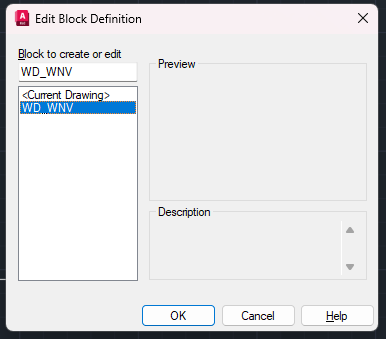
\includegraphics[width=0.5\textwidth]{block_editor_command.png}
              \caption{Block Editor command in AutoCAD Electrical}
          \end{figure}
    \item [\textbf{Significance}] The Block Editor command is essential for creating reusable components in the drawing. It allows users to define and edit blocks for consistent use.
\end{description}


\addcontentsline{toc}{section}{Discussion \& Conclusion}
In this report, we have explored various essential commands in AutoCAD Electrical for creating and modifying electrical drawings. These commands include basic drawing tools like Line, Polyline, Circle, and Arc, as well as editing tools such as Move, Copy, Rotate, and Mirror. Additionally, we covered commands for managing layers, inserting symbols, numbering wires, and creating schematics. Mastering these commands improves productivity and ensures the accuracy of electrical designs.

The detailed descriptions and examples provided for each command demonstrate their usage and significance in electrical design. Commands like Layer and Symbol Insert help organize the drawing and maintain consistency, while Wire Number and Component Tagging enhance clarity and organization. Overall, AutoCAD Electrical offers a comprehensive set of tools that streamline the electrical design process, enabling users to create accurate and efficient drawings, improve workflow, and achieve better project outcomes.

% \bibliographystyle{IEEEtran}
% \renewcommand{\bibname}{References}
% \addcontentsline{toc}{section}{References}
% \bibliography{ref}

\end{document}
